% Created 2026-02-03 Tue 18:23
% Intended LaTeX compiler: pdflatex
\documentclass[aspectratio=1610]{beamer}
\usepackage[utf8]{inputenc}
\usepackage[T1]{fontenc}
\usepackage{graphicx}
\usepackage{longtable}
\usepackage{wrapfig}
\usepackage{rotating}
\usepackage[normalem]{ulem}
\usepackage{amsmath}
\usepackage{amssymb}
\usepackage{capt-of}
\usepackage{hyperref}
\setbeamertemplate{navigation symbols}{}
\setbeamertemplate{footline}[frame number]
\usepackage{tikz}
\usetikzlibrary{shapes,arrows,positioning,shadows,calc}
\usepackage{pgfplots}
\usepgfplotslibrary{polar}
\pgfplotsset{compat=1.18}
\usepackage[height=1200]{beamer-reveal}
\usetheme{Madrid}
\usecolortheme{dolphin}
\usefonttheme{structurebold}
\author{Mohammad Durrani}
\date{\today}
\title{Course Overview and The Shell}
\subtitle{CMSC398W: Practical Tools For Efficient Development}
\hypersetup{
 pdfauthor={Mohammad Durrani},
 pdftitle={Course Overview and The Shell},
 pdfkeywords={},
 pdfsubject={},
 pdfcreator={Emacs 30.2 (Org mode 9.7.11)}, 
 pdflang={English}}
\setbeamertemplate{note page}{\insertnote}
\setbeameroption{show only notes}
\setbeamersize{text margin left=0.25cm, text margin right=0.25cm}
\begin{document}

\maketitle
\section*{About The Class}
\label{sec:orgb9b57d7}

\begin{frame}[label={sec:orgf6b98bc}]{Welcome To Class!}
\end{frame}


\begin{frame}[label={sec:orge4b87ca}]{Icebreaker}
\begin{block}{Please share in the Zoom chat:}
\begin{enumerate}
\item Your year (Freshman, Sophomore, Junior, Senior)
\item Either:
\begin{itemize}
\item One thing you did over break, \alert{OR}
\item What you hope to learn from this class
\end{itemize}
\end{enumerate}
\end{block}
\end{frame}
\note{Note
This is a note.}
\begin{frame}[label={sec:org6548ab6}]{About The Class}
\begin{block}{Course Information}
\alert{CMSC398W: Practical Tools For Efficient Development}

\begin{itemize}
\item Overview of tools used in development: command line, Git, debuggers, build systems, etc.
\item Emphasis on breadth over depth
\item Hands-on learning through projects
\end{itemize}
\end{block}
\begin{exampleblock}{Course Goals}\label{sec:org2c63ae1}
\begin{itemize}
\item Improve your computing ecosystem literacy
\item Improve your efficiency
\item Reduce cognitive load while developing
\end{itemize}
\end{exampleblock}
\end{frame}
\begin{frame}[label={sec:orgb48c77f}]{About Me - Mohammad}
\begin{columns}
\begin{column}{0.55\columnwidth}
\alert{Mohammad Durrani}

\begin{itemize}
\item Senior
\item CS + Math, minor in Robotics
\item \alert{Previous Experience:}
\begin{itemize}
\item Teaching this class since Spring 2025
\item SWE Intern at Google in SF
\item SWE Intern at TRX Systems in Greenbelt
\end{itemize}
\end{itemize}
\end{column}
\begin{column}{0.4\columnwidth}
\alert{Hobbies:}

\begin{itemize}
\item Rock climbing
\item Basketball
\item Robots
\end{itemize}
\end{column}
\end{columns}
\end{frame}
\begin{frame}[label={sec:org3c1eb38}]{What To Expect}
\begin{block}{Course Structure}
\alert{Read the syllabus for all course-related information!}
\end{block}
\begin{columns}
\begin{column}{0.48\columnwidth}
\begin{itemize}
\item Introduction of topic
\item Motivation / real-world example
\item Technical details
\end{itemize}
\end{column}
\begin{column}{0.48\columnwidth}
\begin{itemize}
\item Projects focusing on application
\item Best way to learn: \alert{use them}
\end{itemize}
\end{column}
\end{columns}
\end{frame}
\begin{frame}[label={sec:org2292c28}]{Course Logistics}
\begin{alertblock}{Communication \& Submission}
\begin{itemize}
\item All course communication: \alert{Piazza}
\item All assignments submitted: \alert{Gradescope}
\item \alert{10\% per-day late penalty} (except the last project)
\end{itemize}
\end{alertblock}
\begin{block}{Grade Breakdown}
\begin{center}
\begin{tabular}{lll}
Percentage & Title & Description\\
\hline
80\% & Projects (20\% per) & 4 Major Projects\\
15\% & Application Days (5\% per) & Completion of Application Days\\
5\% & Participation & Participation in class\\
\end{tabular}
\end{center}
\end{block}
\end{frame}
\begin{frame}[label={sec:org670b2f8}]{Application Days}
\begin{block}{Based on Feedback}
Based on feedback from the previous iteration, we'll have days focused on using the tools we learn in class on toy problems.
\end{block}
\begin{exampleblock}<2->{Three Application Days}\label{sec:org26d506c}
\begin{enumerate}
\item \alert{Shell}
\item \alert{Git}
\item \alert{Networking}
\end{enumerate}

\vspace{0.3em}
(Subject to change)
\end{exampleblock}
\end{frame}
\begin{frame}[label={sec:org9e09965}]{Grade Distribution}
\begin{center}
\includegraphics[width=.9\linewidth]{grade-pie.png}
\label{org74e1d05}
\end{center}
\end{frame}
\section*{The Shell}
\label{sec:org2ea57a0}

\begin{frame}[label={sec:org90457f7}]{What is the Shell?}
\begin{definition}[Shell]\label{sec:orge0218ad}
A text-based interface to the operating system.
\end{definition}
\begin{block}<2->{Terminal vs Shell}
\begin{center}
\begin{tabular}{lll}
Component & Role & Examples\\
\hline
\alert{Terminal} & The application that runs the shell & iTerm2, Windows Terminal\\
\alert{Shell} & Interprets and runs commands & bash, zsh, fish\\
\end{tabular}
\end{center}
\end{block}
\end{frame}
\begin{frame}[label={sec:org5c59aff},fragile]{Why Do We Need It?}
 \begin{block}{Power \& Efficiency}
\begin{itemize}[<+->]
\item \alert{Speed:} Automate repetitive tasks
\item \alert{Control:} Do things GUIs simply can't
\item \alert{Remote Machines:} The standard way to manage servers
\end{itemize}
\end{block}
\begin{alertblock}<2->{Why Bash?}
We focus on \alert{Bash} because it's common and the skills are largely transferable.
On macOS the default interactive shell is often \texttt{zsh}, but the core concepts and scripting translate.
\end{alertblock}
\end{frame}
\begin{frame}[label={sec:orgd92011e},fragile]{The Prompt}
 \begin{block}{Anatomy of the Prompt}
\texttt{username@host:directory\$}
\end{block}
\begin{columns}
\begin{column}{1.0\columnwidth}
\begin{center}
\begin{tabular}{ll}
Component & Description\\
\hline
username & Currently logged in user\\
@ & Separator (convention)\\
host & Machine name\\
directory & Current working directory\\
\$ & User-level shell indicator\\
\texttt{\#} & Root-level shell indicator\\
\end{tabular}
\end{center}
\end{column}
\end{columns}
\end{frame}
\begin{frame}[label={sec:org5e5f606},fragile]{Basic Commands}
 \begin{block}{How It Works}
Type command → shell splits on whitespace → runs program with arguments

Prompts vary and are customizable (your \texttt{PS1} controls this).
\end{block}
\begin{exampleblock}<2->{Examples}\label{sec:org4be45af}
\begin{verbatim}
date                    # Show date/time
echo hello              # Print text
echo "Hello World"      # Handle spaces
ls -l ~                # Command with flags
\end{verbatim}
\end{exampleblock}
\end{frame}
\begin{frame}[label={sec:org29b2605},fragile]{File Paths}
 \begin{block}{Types}
\alert{Absolute:} \texttt{/home/user/docs} (from root)

\alert{Relative:} \texttt{../other/file.txt} (from current location)
\end{block}
\begin{exampleblock}<2->{Special Symbols}\label{sec:orgedc1002}
\begin{center}
\begin{tabular}{ll}
Symbol & Meaning\\
\hline
\texttt{.} & Current directory\\
\texttt{..} & Parent directory\\
\texttt{\textasciitilde{}} & Home directory\\
\end{tabular}
\end{center}
\end{exampleblock}
\end{frame}
\begin{frame}[label={sec:org3f910a1},fragile]{Essential Navigation Commands}
 \begin{block}{Why?}
How do you know where you are in a system with millions of files?
\end{block}
\begin{block}<2->{Commands}
\begin{center}
\begin{tabular}{ll}
Command & Description\\
\hline
\texttt{pwd} & Print working directory\\
\texttt{cd <dir>} & Change directory\\
\texttt{ls [dir]} & List directory contents\\
\texttt{ls -l} & Long format listing\\
\texttt{ls -a} & Show hidden files\\
\texttt{ls -lh} & Human-readable sizes\\
\end{tabular}
\end{center}
\end{block}
\end{frame}
\begin{frame}[label={sec:org38a772e},fragile]{Navigation Examples}
 \begin{columns}
\begin{column}{0.48\columnwidth}
\begin{block}{Our Filesystem Structure}
\begin{verbatim}
/ (root)
├── bin/
├── home/
│   └── user/
│       ├── docs/
│       └── photos/
└── usr/
\end{verbatim}
\end{block}
\end{column}
\begin{column}{0.48\columnwidth}
\begin{exampleblock}<2->{Using Navigation Commands}\label{sec:org4c12b05}
\begin{verbatim}
$ pwd
/home/user

$ ls -F          # -F adds / to directories
docs/  photos/

$ cd docs
$ pwd
/home/user/docs

$ cd ..
$ pwd
/home/user
\end{verbatim}
\end{exampleblock}
\end{column}
\end{columns}
\end{frame}
\begin{frame}[label={sec:org42c7d7e},fragile]{Think-Pair-Share: Navigation Puzzle}
 \begin{block}{The Path}
You start in \texttt{/home/user/docs}. You run the following command:

\begin{verbatim}
cd .././photos/../././docs/../../
\end{verbatim}
\end{block}
\begin{exampleblock}{The Question}\label{sec:org030ec48}
Where are you now? Work with a partner to trace the path step-by-step.
\end{exampleblock}
\begin{alertblock}<2->{Answer}
\alert{/home}
\begin{enumerate}[<+->]
\item \texttt{..} \(\rightarrow\) \texttt{/home/user}
\item \texttt{./photos} \(\rightarrow\) \texttt{/home/user/photos}
\item \texttt{..} \(\rightarrow\) \texttt{/home/user}
\item \texttt{././docs} \(\rightarrow\) \texttt{/home/user/docs}
\item \texttt{../../} \(\rightarrow\) \texttt{/home}
\end{enumerate}
\end{alertblock}
\end{frame}
\begin{frame}[label={sec:orgfb7508b},fragile]{File and Directory Manipulation}
 \begin{block}{Common Operations}
\begin{center}
\begin{tabular}{ll}
Command & Description\\
\hline
\texttt{mkdir <dir>} & Make directory\\
\texttt{touch <file>} & Create empty file / update timestamp\\
\texttt{cp <src> <dst>} & Copy files/directories\\
\texttt{mv <src> <dst>} & Move/rename files\\
\texttt{rm <file>} & Remove files\\
\end{tabular}
\end{center}
\end{block}
\begin{alertblock}<2->{What do these flags actually do?}
\begin{itemize}[<+->]
\item \alert{-r}: Recursive (directories)
\item \alert{-i}: Interactive (ask before delete)
\item \alert{-f}: Force (no prompt)
\item \alert{-v}: Verbose (show progress)
\end{itemize}
\end{alertblock}
\end{frame}
\begin{frame}[label={sec:org8fb515c},fragile]{File Manipulation Examples}
 \begin{block}{Examples}
\begin{verbatim}
# Create nested directories
mkdir -p project/src/utils

# Copy a folder and all its contents
cp -r folder1 folder1_backup

# Rename a file
mv old_name.txt new_name.txt

# Remove a folder and its contents (be careful!)
rm -rf temporary_work
\end{verbatim}
\end{block}
\end{frame}
\begin{frame}[label={sec:orgdc1b1a9},fragile]{Time to Explore: File Operations}
 \begin{block}{Challenge}
Perform the following tasks using only the shell:

\begin{enumerate}
\item Create a directory named \texttt{STIC}, and inside it, a directory named \texttt{lab1}.
\item Create three empty files in \texttt{lab1} named \texttt{test1.py}, \texttt{test2.py}, and \texttt{notes.txt}.
\item Copy \texttt{notes.txt} to a new file called \texttt{README.md}.
\item Move all \texttt{.py} files into a new subdirectory called \texttt{src}.
\item Try to remove the \texttt{STIC} directory using \texttt{rmdir}. Why does it fail?
\end{enumerate}
\end{block}
\end{frame}
\begin{frame}<2->[label={sec:orgafc541d},fragile]{Solutions: File Operations}
 \begin{exampleblock}{Steps}\label{sec:orgb76a3eb}
\begin{verbatim}
# 1. Create nested
mkdir -p STIC/lab1

# 2. Create files
touch STIC/lab1/test1.py STIC/lab1/test2.py STIC/lab1/notes.txt

# 3. Copy
cp STIC/lab1/notes.txt STIC/lab1/README.md

# 4. Move
mkdir STIC/lab1/src
mv STIC/lab1/*.py STIC/lab1/src/

# 5. Why fail?
rmdir STIC  # Fails: "Directory not empty"
rm -r STIC  # Use recursive remove instead!
\end{verbatim}
\end{exampleblock}
\end{frame}
\begin{frame}[label={sec:org7d70369},fragile]{Viewing File Contents}
 \begin{block}{Why not just use VS Code?}
What if the file is on a remote server? What if it's 10GB?
\end{block}
\begin{block}<2->{Viewing Commands}
\begin{center}
\begin{tabular}{ll}
Command & Description\\
\hline
\texttt{cat <file>} & Display entire file\\
\texttt{less <file>} & Page through file (q to quit)\\
\texttt{head -n N <file>} & Show first N lines\\
\texttt{tail -n N <file>} & Show last N lines\\
\texttt{tail -f <file>} & Follow file updates (logs)\\
\end{tabular}
\end{center}
\end{block}
\end{frame}
\begin{frame}[label={sec:org864056c},fragile]{Viewing Examples}
 \begin{block}{File Viewing}
\begin{verbatim}
# Display entire file
cat file.txt

# Page through file (Search with /, quit with q)
less file.txt

# First 20 lines
head -n 20 file.txt

# Last 15 lines
tail -n 15 file.txt

# Follow log file as it grows
tail -f /var/log/system.log
\end{verbatim}
\end{block}
\end{frame}
\begin{frame}[label={sec:org50a3bd2},fragile]{Think-Pair-Share: Which tool when?}
 \begin{block}{Match the tool to the task}
\begin{enumerate}
\item You want to see the last 5 errors in a log file.
\item You want to read a 1GB text file without crashing your computer.
\item You want to see the first line of every \texttt{.txt} file in a directory.
\item You want to watch a log file update in real-time as you run a server.
\end{enumerate}
\end{block}
\begin{exampleblock}<2->{Answers}\label{sec:orgc6b9cf6}
\begin{enumerate}[<+->]
\item \texttt{tail -n 5}
\item \texttt{less} (it doesn't load the whole file at once!)
\item \texttt{head -n 1 *.txt}
\item \texttt{tail -f}
\end{enumerate}
\end{exampleblock}
\end{frame}
\begin{frame}[label={sec:orgaa46ae1},fragile]{PATH: Finding Programs}
 \begin{block}{How does the shell know where 'ls' is?}
The \texttt{PATH} environment variable is a list of directories the shell searches through every time you type a command.
\end{block}
\begin{exampleblock}{Key Points}\label{sec:orga95829a}
\begin{itemize}
\item Colon-separated list: \texttt{/usr/local/bin:/usr/bin:/bin}
\item \alert{First match wins:} The shell searches from left to right.
\item If it's not in \texttt{PATH}, use an explicit path (e.g., \texttt{/usr/local/bin/my\_prog} or \texttt{./my\_prog}).
\end{itemize}
\end{exampleblock}
\end{frame}
\begin{frame}[label={sec:org209802c},fragile]{PATH Variable - Example}
 \begin{block}{Exploring PATH}
\begin{verbatim}
# Display your PATH
$ echo $PATH
/usr/local/bin:/usr/bin:/bin:/usr/sbin:/sbin

# Find where a command actually lives (portable)
$ command -v ls
/bin/ls

# Run directly without relying on PATH
$ /bin/date
# sample output: Fri Jan 30 14:00:00 EST 2026
\end{verbatim}
\end{block}
\end{frame}
\begin{frame}[label={sec:org1e76b2b},fragile]{Modifying PATH}
 \begin{exampleblock}{Adding to PATH}\label{sec:org83effdd}
\begin{verbatim}
export PATH="$HOME/my_tools:$PATH"
\end{verbatim}

This adds \texttt{my\_tools} to the beginning of your PATH, giving it priority.
\end{exampleblock}
\begin{alertblock}<2->{Rhetorical Question}
Why might it be dangerous to add \texttt{.} (current directory) to the \alert{start} of your PATH?
\end{alertblock}
\end{frame}
\begin{frame}[label={sec:org558a4c2},fragile]{Environment Variables}
 \begin{columns}
\begin{column}{0.48\columnwidth}
\begin{definition}[Definition]\label{sec:orgaa2da59}
Variables that define the environment in which your programs run.
\end{definition}
\begin{block}{Common Variables}
\begin{center}
\begin{tabular}{ll}
Var & Meaning\\
\hline
\texttt{PATH} & Command search\\
\texttt{HOME} & Home directory\\
\texttt{USER} & Username\\
\texttt{PWD} & Current dir\\
\end{tabular}
\end{center}
\end{block}
\end{column}
\begin{column}{0.48\columnwidth}
\begin{block}{Usage Examples}
\begin{verbatim}
# Display
echo $USER

# Set (local to shell)
MY_VAR="value"

# Export (available to child procs)
export MY_VAR="value"

# View all
env | head
\end{verbatim}
\end{block}
\end{column}
\end{columns}
\end{frame}
\begin{frame}[label={sec:org74dbb96},fragile]{Time to Explore: Environment}
 \begin{block}{Challenge}
\begin{enumerate}
\item Type \texttt{env} and look at the output. Can you find \texttt{SHELL} and \texttt{PWD}?
\item Create a variable: \texttt{MY\_NAME}"Your Name"\texttt{. Try =echo \$MY\_NAME}.
\item Open a \alert{new} terminal window. Is \texttt{\$MY\_NAME} still there?
\item Try \texttt{export PS1}"Ready> "= (or something fun). What happened to your prompt?
\end{enumerate}
\end{block}
\end{frame}
\begin{frame}<2->[label={sec:org18137cf},fragile]{Solutions: Environment}
 \begin{exampleblock}{Key Takeaways}\label{sec:orge318c3d}
\begin{itemize}[<+->]
\item \alert{Ephemeral:} Variables die when the terminal is closed.
\item \alert{Local vs Export:} Without \texttt{export}, child programs (like scripts you run) can't see the variable.
\item \alert{Customization:} \texttt{PS1} is the variable that controls what your prompt looks like!
\end{itemize}
\end{exampleblock}
\end{frame}
\section*{Shell Tools}
\label{sec:orgb6175c3}

\begin{frame}[label={sec:orgd2d1abe},fragile]{Searching and Finding}
 \begin{block}{Why search from the CLI?}
Imagine searching through 100,000 lines of logs or finding a specific file in a project with 50 subdirectories.
\end{block}
\begin{block}<2->{Search Commands}
\begin{center}
\begin{tabular}{lll}
Command & Description & Useful Flags\\
\hline
\texttt{find} & Find files & \texttt{-name}, \texttt{-type}, \texttt{-size}\\
\texttt{grep} & Search text & \texttt{-r} (recursive), \texttt{-i} (case), \texttt{-n} (line\#)\\
\texttt{which} & Find exe & -\\
\end{tabular}
\end{center}
\end{block}
\end{frame}
\begin{frame}[label={sec:orgf5ff7d8},fragile]{find: Locate Files}
 \begin{block}{Examples with Output}
\begin{verbatim}
$ find . -name "*.txt"
./notes.txt
./data/results.txt

# Find directories only
$ find . -type d -name "test*"
./project/tests

# Find files larger than 100MB
$ find /var/log -size +100M
\end{verbatim}
\end{block}
\end{frame}
\begin{frame}[label={sec:org98168ae},fragile]{grep: Search File Contents}
 \begin{block}{Examples}
\begin{verbatim}
$ grep "error" app.log
Connection error at 10:32

# Show line numbers (-n)
$ grep -n "error" app.log
15:Connection error at 10:32

# Recursive search (-r) in a directory
$ grep -r "TODO" src/
src/main.py: # TODO: optimize this

# Case-insensitive (-i)
$ grep -i "ERROR" app.log
\end{verbatim}
\end{block}
\end{frame}
\begin{frame}[label={sec:org82c74a8},fragile]{Think-Pair-Share: The Needle in the Haystack}
 \begin{block}{The Challenge}
You are working on a massive project. You need to find a "TODO" comment related to "authentication" in any file.

\alert{\alert{Task:}} How would you find this line using only \texttt{grep}? Discuss with your neighbor the flags you'd need.
\end{block}
\begin{alertblock}<2->{Possible Solution}
\begin{verbatim}
$ grep -rn "TODO.*authentication" .
\end{verbatim}

\begin{itemize}
\item \alert{-r}: Search all files in all subdirectories.
\item \alert{-n}: Tell me exactly which line the comment is on!
\end{itemize}
\end{alertblock}
\end{frame}
\begin{frame}[label={sec:org0eb0ee7},fragile]{Wildcards and Globbing}
 \begin{block}{Glob Patterns}
\begin{center}
\begin{tabular}{ll}
Pattern & Matches\\
\hline
\texttt{*} & Any string (including empty)\\
\texttt{?} & Any single character\\
\texttt{[abc]} & Any character in brackets\\
\texttt{[a-z]} & Any character in range\\
\end{tabular}
\end{center}
\end{block}
\end{frame}
\begin{frame}[label={sec:org15d25dd},fragile]{Globbing Examples}
 \begin{block}{Basic Wildcards}
\begin{verbatim}
# All .txt files
ls *.txt

# Files starting with 'test'
ls test*

# Single character: matches file1.txt but not file10.txt
ls file?.txt
\end{verbatim}
\end{block}
\end{frame}
\begin{frame}[label={sec:org7887512},fragile]{Globbing Examples - Advanced}
 \begin{block}{Character Sets and Negation}
\begin{verbatim}
# Match specific numbers
ls file[123].txt

# Match any lowercase letter
ls [a-z]*.txt

# Negation: anything NOT starting with a-z
ls [!a-z]*
\end{verbatim}
\end{block}
\end{frame}
\begin{frame}[label={sec:org68bd5ca},fragile]{Time to Explore: Globbing}
 \begin{block}{Files in Directory}
\texttt{img1.png}, \texttt{img10.png}, \texttt{img2.png}, \texttt{image.png}, \texttt{backup\_img1.png}
\end{block}
\begin{exampleblock}{Predict}\label{sec:org735de1c}
Which files match these patterns?
\begin{enumerate}
\item \texttt{img?.png}
\item \texttt{img*.png}
\item \texttt{img[1-9].png}
\item \texttt{*img1.png}
\end{enumerate}
\end{exampleblock}
\begin{alertblock}<2->{Answers}
\begin{enumerate}[<+->]
\item \texttt{img1.png}, \texttt{img2.png}
\item \texttt{img1.png}, \texttt{img10.png}, \texttt{img2.png}
\item \texttt{img1.png}, \texttt{img2.png}
\item \texttt{img1.png}, \texttt{backup\_img1.png}
\end{enumerate}
\end{alertblock}
\end{frame}
\begin{frame}[label={sec:org1c4e493},fragile]{Brace Expansion}
 \begin{definition}[Creating Multiple Arguments]\label{sec:orgde064d7}
Brace expansion generates multiple strings from a pattern. Excellent for bulk creation.
\end{definition}
\begin{block}{Examples}
\begin{verbatim}
# Create multiple files at once
touch file{1,2,3}.txt
# Creates: file1.txt, file2.txt, file3.txt

# Ranges
echo {1..10}
echo {a..z}

# Nested expansion
mkdir -p project/{src,test,docs}
\end{verbatim}
\end{block}
\end{frame}
\begin{frame}[label={sec:org90ef838},fragile]{Command History}
 \begin{block}{History Features}
\begin{center}
\begin{tabular}{ll}
Key/Command & Action\\
\hline
Up/Down arrows & Navigate history\\
\texttt{history} & Show command history\\
\texttt{!!} & Repeat last command\\
\texttt{!grep} & Execute last command starting with grep\\
Ctrl+R & Reverse search history (The MVP!)\\
\end{tabular}
\end{center}
\end{block}
\end{frame}
\begin{frame}[label={sec:org0ef2dcf},fragile]{History Examples}
 \begin{block}{Using History}
\begin{verbatim}
# View last 20 commands
history 20

# Forgot sudo?
$ ls /var/root
ls: /var/root: Permission denied
$ sudo !!

# Search history
(Press Ctrl+R, then type 'ssh')
(reverse-i-search)`ssh': ssh user@umd.edu
\end{verbatim}
\end{block}
\end{frame}
\begin{frame}[label={sec:org77dc55a},fragile]{Tab Completion}
 \begin{exampleblock}{Productivity Booster}\label{sec:org7559290}
\alert{Tab completion} saves time and prevents typos. If you aren't mashing the Tab key, you're working too hard.
\end{exampleblock}
\begin{block}{How it works}
\begin{itemize}[<+->]
\item Press \texttt{Tab} once to complete a unique match.
\item Press \texttt{Tab} twice to see all possibilities if it's ambiguous.
\item Example: \texttt{cd /u[TAB]l[TAB]b[TAB]} \(\rightarrow\) \texttt{cd /usr/local/bin/}
\end{itemize}
\end{block}
\end{frame}
\begin{frame}[label={sec:orgf2dd0cd}]{Command Substitution}
\begin{definition}[Using Command Output]\label{sec:orgd2f3849}
Command substitution allows you to use the output of a command as an argument to another command.
\end{definition}
\end{frame}
\begin{frame}[label={sec:org102bb11}]{Command Substitution Execution Order}
\begin{block}{How It Works}
\begin{center}
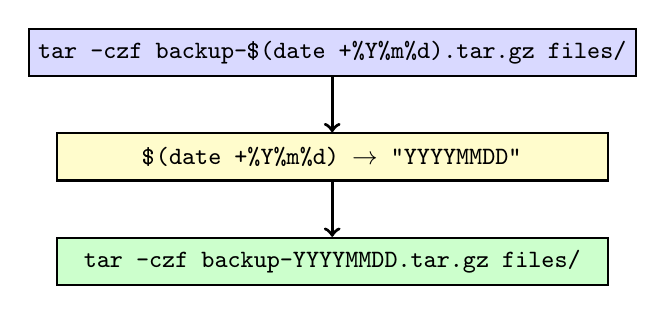
\begin{tikzpicture}[
    node distance=0.7cm,
    box/.style={rectangle, draw, thick, minimum width=7cm, minimum height=0.6cm, align=center, font=\small\ttfamily}
]
    \node[box, fill=blue!15] (original) {tar -czf backup-\$(date +\%Y\%m\%d).tar.gz files/};
    \node[box, fill=yellow!20, below=of original] (executed) {\$(date +\%Y\%m\%d) $\rightarrow$ "YYYYMMDD"};
    \node[box, fill=green!20, below=of executed] (final) {tar -czf backup-YYYYMMDD.tar.gz files/};

    \draw[->, very thick] (original) -- (executed);
    \draw[->, very thick] (executed) -- (final);
\end{tikzpicture}
\end{center}

Inner command executes → output replaces substitution → full command runs
\end{block}
\end{frame}
\begin{frame}[label={sec:org1a4be1f},fragile]{Command Substitution Examples}
 \begin{block}{Substitution Syntax}
\begin{verbatim}
# Using $(command) syntax (preferred)
echo "Today is $(date)"
files=$(ls -1)
echo "Found $(wc -l < file.txt) lines"

# Using backticks (older syntax)
echo "Today is `date`"

# Nested substitution
echo "User $(whoami) in $(pwd)"
\end{verbatim}
\end{block}
\end{frame}
\begin{frame}[label={sec:org107587e},fragile]{Think-Pair-Share: Creative Substitution}
 \begin{block}{Scenario}
You want to create a directory named after the current year and month, and then move all your \texttt{.log} files into it.
\end{block}
\begin{exampleblock}{Challenge}\label{sec:org6dd2c1c}
How can you do this in one or two lines using command substitution? (Hint: check \texttt{man date})
\end{exampleblock}
\begin{alertblock}<2->{Answer}
\begin{verbatim}
mkdir "$(date +%Y-%m)"
mv *.log "$(date +%Y-%m)"
\end{verbatim}
\end{alertblock}
\end{frame}
\section*{Pipes and Redirection}
\label{sec:org0b65efc}

\begin{frame}[label={sec:org16185fd},fragile]{Redirection Basics}
 \begin{columns}
\begin{column}{0.35\columnwidth}
\begin{block}{Problem}
Output goes to screen and disappears
\end{block}
\end{column}
\begin{column}{0.6\columnwidth}
\begin{exampleblock}{Solution}\label{sec:orgc31c962}
\begin{center}
\begin{tabular}{ll}
Operator & Action\\
\hline
\texttt{>} & Overwrite file\\
\texttt{>{}>{}} & Append to file\\
\texttt{2>} & Redirect errors\\
\texttt{\&>} & Redirect everything\\
\end{tabular}
\end{center}

Note: \texttt{command \&> file} works in bash/zsh; the portable form is \texttt{command > file 2>\&1}.
\end{exampleblock}
\end{column}
\end{columns}
\end{frame}
\begin{frame}[label={sec:org5bc85a8},fragile]{File Descriptors \& Redirection}
 \begin{block}{Visual Model}
\begin{center}
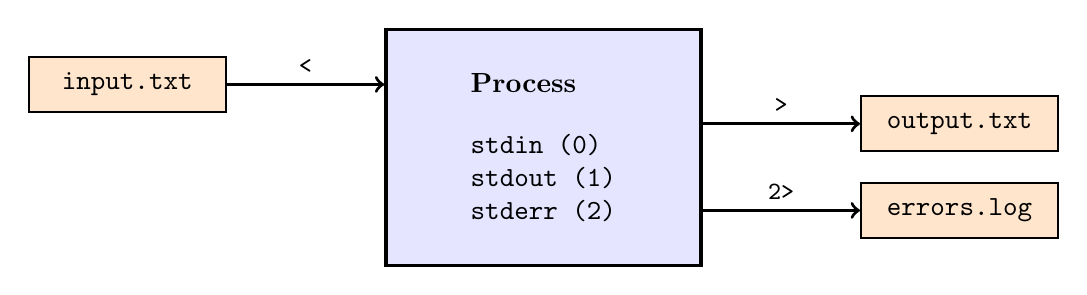
\begin{tikzpicture}[
    node distance=0.3cm,
    process/.style={rectangle, draw, very thick, minimum width=4cm, minimum height=3cm, align=left, fill=blue!10},
    file/.style={rectangle, draw, thick, minimum width=2.5cm, minimum height=0.7cm, align=center, fill=orange!20},
    label/.style={font=\small\ttfamily}
]
    % Process box
    \node[process] (proc) at (0,0) {
        \textbf{Process}\\[1em]
        \texttt{stdin  (0)}\\
        \texttt{stdout (1)}\\
        \texttt{stderr (2)}
    };

    % Input file
    \node[file, left=2cm of proc, yshift=0.8cm] (input) {\texttt{input.txt}};

    % Output file
    \node[file, right=2cm of proc, yshift=0.3cm] (output) {\texttt{output.txt}};

    % Error file
    \node[file, right=2cm of proc, yshift=-0.8cm] (errors) {\texttt{errors.log}};

    % Arrows
    \draw[->, very thick] (input.east) -- node[above, label] {\texttt{<}} (proc.west |- input);
    \draw[->, very thick] (proc.east |- output) -- node[above, label] {\texttt{>}} (output.west);
    \draw[->, very thick] (proc.east |- errors) -- node[above, label] {\texttt{2>}} (errors.west);
\end{tikzpicture}
\end{center}

\begin{itemize}[<+->]
\item \texttt{command > file} → stdout to file
\item \texttt{command 2>\&1} → stderr to stdout
\item \texttt{command \&> file} → both to file
\end{itemize}
\end{block}
\end{frame}
\begin{frame}[label={sec:orgb45feaa},fragile]{Redirection Examples}
 \begin{block}{Using Redirection}
\begin{verbatim}
# Redirect output to file
echo "Hello" > output.txt
ls -l >> listing.txt

# Redirect input
sort < unsorted.txt

# Redirect errors
command 2> errors.log

# Combine stdout and stderr
command > all.log 2>&1
command &> all.log  # Shorter syntax
\end{verbatim}
\end{block}
\end{frame}
\begin{frame}[label={sec:org50a414d},fragile]{Capturing Errors vs Output}
 \begin{block}{Debugging Example}
\begin{verbatim}
# Script that produces both stdout and stderr
$ python buggy_script.py
Processing file1.txt
ERROR: file2.txt not found
Done

# Capture separately
$ python buggy_script.py > output.txt 2> errors.txt

$ cat output.txt
Processing file1.txt
Done

$ cat errors.txt
ERROR: file2.txt not found
\end{verbatim}
\end{block}
\end{frame}
\begin{frame}[label={sec:org38a8761},fragile]{Think-Pair-Share: Redirection Pitfalls}
 \begin{block}{Sequence}
\begin{verbatim}
echo "Hello" > greeting.txt
echo "World" >> greeting.txt
echo "Goodbye" > greeting.txt
cat greeting.txt
\end{verbatim}
\end{block}
\begin{exampleblock}{Discussion}\label{sec:org6fb99fa}
\begin{enumerate}
\item What is the final content of \texttt{greeting.txt}?
\item What happens if you run \texttt{cat greeting.txt > greeting.txt}? \alert{WARNING: Don't do this yet!}
\item How can you save both errors and output to the same file?
\end{enumerate}
\end{exampleblock}
\begin{alertblock}<2->{Answer}
\begin{enumerate}[<+->]
\item \alert{Goodbye} (The final \texttt{>} nuked previous content).
\item The file becomes \alert{empty}! (The shell truncates the file for writing before \texttt{cat} can read it).
\item \texttt{command \&> file}
\end{enumerate}
\end{alertblock}
\end{frame}
\begin{frame}[label={sec:org52d6b7a},fragile]{Pipes}
 \begin{columns}
\begin{column}{0.48\columnwidth}
\begin{block}{Problem}
Count .txt files:
\begin{itemize}
\item \texttt{ls} shows files
\item \texttt{grep} filters
\item \texttt{wc -l} counts
\end{itemize}

How to connect?
\end{block}
\end{column}
\begin{column}{0.48\columnwidth}
\begin{exampleblock}{Solution}\label{sec:orgc7d8ba1}
Use pipes (\texttt{|})

\begin{verbatim}
ls -l | grep txt | wc -l
\end{verbatim}
\end{exampleblock}
\end{column}
\end{columns}
\begin{alertblock}<2->{Philosophy}
"Do one thing well" — combine simple tools for complex tasks
\end{alertblock}
\end{frame}
\begin{frame}[label={sec:orgdcce901}]{How Pipes Work (Visual)}
\begin{block}{Data Flow}
\begin{center}
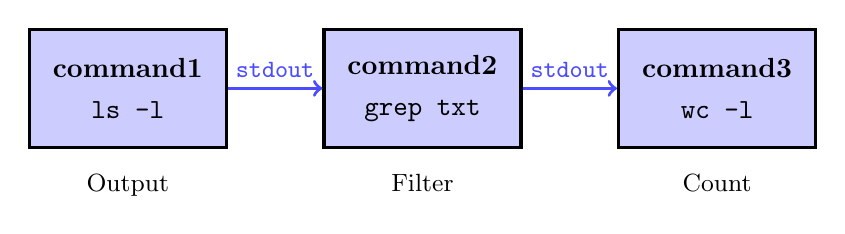
\begin{tikzpicture}[
    node distance=1.2cm,
    cmd/.style={rectangle, draw, very thick, minimum width=2.5cm, minimum height=1.5cm, align=center, fill=blue!20},
    pipe/.style={->, very thick, blue!70}
]
    % Commands
    \node[cmd] (cmd1) {\textbf{command1}\\[0.3em]\texttt{ls -l}};
    \node[cmd, right=of cmd1] (cmd2) {\textbf{command2}\\[0.3em]\texttt{grep txt}};
    \node[cmd, right=of cmd2] (cmd3) {\textbf{command3}\\[0.3em]\texttt{wc -l}};

    % Labels below
    \node[below=0.2cm of cmd1, font=\small] {Output};
    \node[below=0.2cm of cmd2, font=\small] {Filter};
    \node[below=0.2cm of cmd3, font=\small] {Count};

    % Pipes
    \draw[pipe] (cmd1.east) -- node[above, font=\small\ttfamily] {stdout} (cmd2.west);
    \draw[pipe] (cmd2.east) -- node[above, font=\small\ttfamily] {stdout} (cmd3.west);
\end{tikzpicture}
\end{center}

Each command runs simultaneously! Data flows left-to-right.\\
stdout of left becomes stdin of right.
\end{block}
\end{frame}
\begin{frame}[label={sec:org9335c9c},fragile]{Pipe Examples}
 \begin{block}{Basic Piping}
\begin{verbatim}
# Count entries in directory listing
ls -1 | wc -l

# Search and sort
cat file.txt | grep "pattern" | sort

# Find largest files
du -h | sort -rh | head -10

# Process logs
cat access.log | grep "404" | wc -l
\end{verbatim}
\end{block}
\begin{alertblock}<2->{Career Note}
Data pipelines are used everywhere: ETL jobs, log analysis, build systems.
\end{alertblock}
\end{frame}
\begin{frame}[label={sec:org2b564ce},fragile]{Building Pipes Step-by-Step}
 \begin{block}{Progressive Example}
\begin{verbatim}
# 1. See all lines
$ cat app.log
ERROR: connection failed
INFO: started successfully
ERROR: timeout

# 2. Filter errors only
$ cat app.log | grep ERROR
ERROR: connection failed
ERROR: timeout

# 3. Count errors
$ cat app.log | grep ERROR | wc -l
2
\end{verbatim}
\end{block}
\end{frame}
\begin{frame}[label={sec:org515477a},fragile]{Think-Pair-Share: Debug the Pipeline}
 \begin{block}{The Goal}
Find all lines with "Error" in \texttt{app.log} and count them.
\end{block}
\begin{exampleblock}{Broken Commands}\label{sec:orgfd47812}
Identify the flaw in each command:
\begin{enumerate}
\item \texttt{grep "Error" app.log > wc -l}
\item \texttt{cat app.log | grep Error | wc}
\end{enumerate}
\end{exampleblock}
\begin{alertblock}<2->{Answers}
\begin{enumerate}[<+->]
\item \alert{Redirection Error:} \texttt{>} sends output to a \alert{file} named \texttt{wc}. Use \texttt{|} to send to a \alert{program}.
\item \alert{Ambiguous Output:} \texttt{wc} shows lines, words, AND characters. Use \texttt{wc -l} for just lines.
\end{enumerate}
\end{alertblock}
\end{frame}
\section*{xargs}
\label{sec:orge5a0e63}

\begin{frame}[label={sec:orge3a5cde},fragile]{xargs: Bridging the Gap}
 \begin{definition}[What is it?]\label{sec:orge01f27c}
\texttt{xargs} builds and executes command lines from standard input. It converts lines of text into \alert{arguments} for another command.
\end{definition}
\begin{block}<2->{Why do we need it?}
Some commands (like \texttt{rm}, \texttt{mkdir}, \texttt{mv}) don't read from standard input. They only accept arguments. \texttt{xargs} bridges this gap.
\end{block}
\end{frame}
\begin{frame}[label={sec:orge4edf8e},fragile]{xargs: Usage and Options}
 \begin{block}{Examples}
\begin{verbatim}
# Delete all .tmp files (safe with spaces)
find . -name "*.tmp" -print0 | xargs -0 rm

# Run 1 command per input line (NUL-delimited)
printf '%s\0' dir1 dir2 dir3 | xargs -0 -n 1 mkdir

# Custom placement of arguments (safe with spaces)
find . -maxdepth 1 -name "*.txt" -print0 | xargs -0 -I {} mv "{}" backup/
\end{verbatim}
\end{block}
\begin{exampleblock}<2->{Common Flags}\label{sec:org6389170}
\begin{center}
\begin{tabular}{ll}
Option & Description\\
\hline
\texttt{-n N} & Use at most N args per command\\
\texttt{-I \{\}} & Replace \{\} with the input string\\
\texttt{-0} & Read NUL-delimited input (safe)\\
\texttt{-P N} & Run N processes in parallel (Fast!)\\
\end{tabular}
\end{center}
\end{exampleblock}
\end{frame}
\begin{frame}[label={sec:org3499da7},fragile]{System Health with top}
 \begin{block}{Monitoring System Resources}
\texttt{top} displays real-time system statistics: CPU, memory, running processes.

\begin{verbatim}
# macOS: Run top once and exit immediately
$ top -l 1 -n 0
\end{verbatim}

\alert{Flags:} \texttt{-l 1} runs top once (1 iteration). \texttt{-n 0} displays 0 processes (header stats only).
\end{block}
\begin{exampleblock}<2->{Common Use Case}\label{sec:org0285027}
Capture CPU and memory usage in scripts for logging or alerting.
\end{exampleblock}
\end{frame}
\begin{frame}[label={sec:orgfa1afbf}]{Section 3: Data Wrangling}
\begin{block}{The Goal}
"Most of your time as a developer is spent moving data from one format to another."
\end{block}
\begin{exampleblock}{Key Objectives}\label{sec:org9e8021c}
\begin{itemize}
\item Transform "messy" logs into structured reports.
\item Clean and filter large datasets without opening heavy editors.
\item Build automated pipelines for repetitive processing.
\end{itemize}
\end{exampleblock}
\end{frame}
\begin{frame}[label={sec:org856e9dd},fragile]{Data Wrangling Overview}
 \begin{columns}
\begin{column}{0.45\columnwidth}
\begin{block}{}
Cleaning, transforming, and analyzing data using command-line tools.

\alert{Tasks:}
\begin{itemize}
\item Extract fields
\item Count frequencies
\item Filter \& Transform
\item Reformat output
\end{itemize}
\end{block}
\end{column}
\begin{column}{0.5\columnwidth}
\begin{block}{}
\begin{itemize}
\item \alert{Filtering:} \texttt{grep}, \texttt{head}, \texttt{tail}
\item \alert{Sorting:} \texttt{sort}, \texttt{uniq}
\item \alert{Editing:} \texttt{sed}, \texttt{awk}, \texttt{tr}
\item \alert{Stats:} \texttt{wc}
\end{itemize}
\end{block}
\end{column}
\end{columns}
\end{frame}
\begin{frame}[label={sec:org5f258db},fragile]{Sorting and Uniqueness (sort, uniq)}
 \begin{alertblock}{Why?}
\texttt{uniq} only works on \alert{adjacent} lines. That's why we almost always \texttt{sort} before we \texttt{uniq}.
\end{alertblock}
\begin{block}<2->{Examples with Output}
\begin{verbatim}
# Sample file: fruits.txt (apple, banana, apple, cherry, banana)

# Count unique occurrences
$ sort fruits.txt | uniq -c
   2 apple
   2 banana
   1 cherry

# Sort by frequency (descending)
$ sort fruits.txt | uniq -c | sort -rn
   2 banana
   2 apple
   1 cherry
\end{verbatim}
\end{block}
\end{frame}
\begin{frame}[label={sec:org6c6d847},fragile]{Data Wrangling Example}
 \begin{block}{Real-World Pipeline}
\begin{verbatim}
# Analyze web server logs
# Find most common ERROR messages
cat access.log \
  | grep "ERROR" \
  | awk '{print $5}' \
  | sort \
  | uniq -c \
  | sort -rn \
  | head -10
\end{verbatim}
\end{block}
\begin{block}{Analysis}
\begin{enumerate}
\item \alert{Read:} Opens the log file.
\item \alert{Filter:} Keeps only ERROR lines.
\item \alert{Extract:} Pulls the 5th column (the error type).
\item \alert{Sort:} Groups identical messages.
\item \alert{Count:} Counts unique occurrences.
\item \alert{Rank:} Sorts by frequency.
\item \alert{Top 10:} Shows the most common errors.
\end{enumerate}
\end{block}
\end{frame}
\begin{frame}[label={sec:org2c85f31},fragile]{Regular Expressions (Regex)}
\begin{block}{Why Regex?}
Regex patterns allow for powerful, flexible text matching beyond simple wildcards.
\end{block}
\end{frame}
\begin{frame}[label={sec:org58ef5b0},fragile]{Regex Flavors: A Shell Caveat}
 \begin{block}{Comparison}
\begin{center}
\begin{tabular}{llll}
Feature & BRE (Basic) & ERE (Extended) & PCRE (Perl/JS/Py)\\
\hline
Tools & \texttt{grep}, \texttt{sed} & \texttt{grep -E}, \texttt{awk} & \texttt{grep -P}, Python\\
\texttt{+}, \texttt{?} & Need \texttt{\textbackslash{}} & Raw: \texttt{+}, \texttt{?} & Raw: \texttt{+}, \texttt{?}\\
\texttt{()}, \texttt{\{\}} & Need \texttt{\textbackslash{}} & Raw: \texttt{()}, \texttt{\{\}} & Raw: \texttt{()}, \texttt{\{\}}\\
\end{tabular}
\end{center}

\begin{itemize}[<+->]
\item \alert{Note:} macOS BSD \texttt{grep} usually lacks \texttt{-P}. Prefer \texttt{grep -E} or install GNU \texttt{grep} (often \texttt{ggrep}).
\end{itemize}
\end{block}
\begin{exampleblock}{Example: Matching "1 or more"}\label{sec:org189b4f5}
\begin{itemize}
\item \alert{BRE:} \texttt{grep 'a\textbackslash{}+'}
\item \alert{ERE:} \texttt{grep -E 'a+'}
\item \alert{PCRE:} \texttt{grep -P 'a+'}
\end{itemize}
\end{exampleblock}
\end{frame}
\begin{frame}[label={sec:org68d219f},fragile]{Pattern Cheat Sheet}
 \begin{center}
\begin{tabular}{lll}
Type & Pattern & Matches\\
\hline
\alert{Anchors} & \texttt{\textasciicircum{}} / \texttt{\$} & Start / End of line\\
\alert{Quantify} & \texttt{*} / \texttt{+} & Zero+ / One+ repetitions\\
\alert{Groups} & \texttt{[]} / \texttt{()} & Sets / Capture groups\\
\alert{Wildcard} & \texttt{.} & Any single character\\
\end{tabular}
\end{center}
\begin{exampleblock}<2->{Basic Examples}\label{sec:org5bb71c4}
\begin{itemize}[<+->]
\item \texttt{\textasciicircum{}apple} matches "apple pie" but not "red apple"
\item \texttt{dog\$} matches "hot dog" but not "dogwood"
\item \texttt{ba+na} matches "banana", "baana", but not "bana"
\item \texttt{[0-9]\{3\}} matches exactly three digits
\end{itemize}
\end{exampleblock}
\end{frame}
\section*{sed (Stream Editor)}
\label{sec:org195f793}

\begin{frame}[label={sec:org0436f54},fragile]{The sed Execution Model}
 \begin{block}{The sed Cycle}
\begin{center}
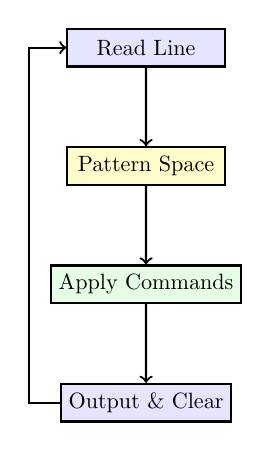
\begin{tikzpicture}[
    scale=0.8, every node/.style={scale=0.8},
    node distance=1cm,
    box/.style={rectangle, draw, thick, minimum width=2.5cm, minimum height=0.6cm, align=center, fill=blue!10},
    arrow/.style={->, thick}
]
    \node[box] (read) {Read Line};
    \node[box, below=of read, fill=yellow!20] (pattern) {Pattern Space};
    \node[box, below=of pattern, fill=green!10] (command) {Apply Commands};
    \node[box, below=of command] (output) {Output \& Clear};

    \draw[arrow] (read) -- (pattern);
    \draw[arrow] (pattern) -- (command);
    \draw[arrow] (command) -- (output);
    \draw[arrow] (output.west) -- ++(-0.5,0) |- (read.west);
\end{tikzpicture}
\end{center}
\end{block}
\begin{alertblock}<2->{Key Concept}
\texttt{sed} works line-by-line. It never modifies the original file unless you use the \texttt{-i} (in-place) flag.
\end{alertblock}
\end{frame}
\begin{frame}[label={sec:org1457b3b},fragile]{sed: Search and Replace}
 \begin{block}{Examples with Output}
\begin{verbatim}
# Replace first 'foo' with 'bar'
$ echo "foo foo" | sed 's/foo/bar/'
bar foo

# Replace ALL 'foo' with 'bar' (global)
$ echo "foo foo" | sed 's/foo/bar/g'
bar bar

# Delete lines matching a pattern
$ printf "line1\n#comment\nline2" | sed '/^#/d'
line1
line2
\end{verbatim}
\end{block}
\end{frame}
\begin{frame}[label={sec:org05d8ec8},fragile]{sed: Addressing and Ranges}
 \begin{block}{Target Specific Lines}
\begin{verbatim}
# Delete only the first 2 lines
$ sed '1,2d' file.txt

# Print only lines 5 through 10
$ sed -n '5,10p' file.txt

# Substitute only on lines containing 'error'
$ sed '/error/s/false/true/' log.txt
\end{verbatim}
\end{block}
\begin{exampleblock}{Practice: config cleanup}\label{sec:org2a90bc6}
\begin{enumerate}
\item Task: Remove all comments (\texttt{\#}) and empty lines from a file.
\end{enumerate}
\end{exampleblock}
\begin{alertblock}<2->{Answer}
\texttt{sed -e '/\textasciicircum{}\#/d' -e '/\textasciicircum{}\$/d' config.txt}
\end{alertblock}
\end{frame}
\begin{frame}[label={sec:org4ffbee3},fragile]{More sed Examples}
 \begin{block}{Advanced Usage}
\begin{verbatim}
# Change delimiter (useful for paths)
sed 's|/usr/local|/opt|g' paths.txt

# Backreferences (Swap first two words)
echo "Hello World" | sed 's/\(\w\+\) \(\w\+\)/\2 \1/'

# Multiple commands
sed -e 's/foo/bar/g' -e 's/baz/qux/g' file.txt

# In-place editing (GNU/BSD differ; macOS needs -i '')
sed -i.bak 's/debug/info/g' config.yml
\end{verbatim}
\end{block}
\end{frame}
\section*{awk (Pattern Processing)}
\label{sec:orgb3e2641}

\begin{frame}[label={sec:org71f53e7},fragile]{awk: The Pattern-Action Model}
 \begin{block}{How it works}
\texttt{awk} automatically loops over every line. You define \alert{patterns} and \alert{actions}.

\centering \large \texttt\{awk 'pattern \{ action \}' file\}
\end{block}
\begin{exampleblock}<2->{Basic Examples}\label{sec:org87c9a29}
\begin{verbatim}
# Print 1st and 3rd columns (default delimiter: space)
$ awk '{print $1, $3}' data.txt

# Filter by value: print line if 2nd col > 100
$ awk '$2 > 100' data.txt

# Use a custom delimiter (e.g., colon)
$ awk -F':' '{print $1}' /etc/passwd
\end{verbatim}
\end{exampleblock}
\end{frame}
\begin{frame}[label={sec:orga76c903},fragile]{awk: Context and Math}
 \begin{block}{Built-in Variables}
\begin{itemize}
\item \alert{\alert{NR:}} Number of Records (Line Number)
\item \alert{\alert{NF:}} Number of Fields (Columns in current line)
\item \alert{\alert{\$0:}} The entire line
\end{itemize}
\end{block}
\begin{exampleblock}<2->{Examples with Output}\label{sec:orgc5e587b}
\begin{verbatim}
# Print line number and the line
$ awk '{print NR, $0}' file.txt

# Sum values in the first column
$ awk '{sum += $1} END {print "Total:", sum}' numbers.txt
Total: 450

# Calculate average of 1st column
$ awk '{s+=$1; c++} END {print "Avg:", s/c}' numbers.txt
\end{verbatim}
\end{exampleblock}
\end{frame}
\begin{frame}[label={sec:orgf11d374},fragile]{Practice: Data Extraction}
 \begin{block}{Challenge}
You have a CSV (\texttt{Name,Age,Score}) called \texttt{class.csv}.
\begin{enumerate}
\item Print only the names of students older than 20.
\item Calculate the total number of words in a text file.
\end{enumerate}
\end{block}
\begin{alertblock}<2->{Answers}
\begin{enumerate}[<+->]
\item \texttt{awk -F',' '\$2 > 20 \{print \$1\}' class.csv}
\item \texttt{awk '\{total +} NF\} END \{print total\}' file.txt=
\end{enumerate}
\end{alertblock}
\end{frame}
\begin{frame}[label={sec:orga55adc4},fragile]{More awk Examples}
 \begin{block}{Advanced Features}
\begin{verbatim}
# Formatted printing (printf)
awk '{printf "Name: %-10s ID: %03d\n", $1, $2}' students.txt

# Length of string
awk 'length($0) > 80' file.txt  # Print lines > 80 chars

# Logical conditions (AND/OR)
awk '$1 == "POST" && $9 == 200' access.log

# Range pattern (start, end)
awk '/START/,/END/' data.txt

# Filter by timestamp range and format output
awk '$1 >= "2026-01-20" && $1 <= "2026-01-25" \
  {printf "[%s %s] %s\n", $1, $2, substr($0, index($0,$3))}' system.log
\end{verbatim}
\end{block}
\end{frame}
\section*{Shell Scripting}
\label{sec:orgd9b136e}

\begin{frame}[label={sec:org0714907},fragile]{Scripting Basics}
 \begin{columns}
\begin{column}{0.45\columnwidth}
\begin{block}{}
\begin{itemize}
\item Automate repetitive tasks
\item Combine multiple commands
\item Add logic (if/loops)
\item Reproducibility
\end{itemize}
\end{block}
\end{column}
\begin{column}{0.5\columnwidth}
\begin{verbatim}
#!/bin/bash
# hello.sh
echo "Hello, $USER!"
echo "Date: $(date)"
\end{verbatim}
\end{column}
\end{columns}
\begin{exampleblock}{Making it Executable}\label{sec:orgaab8643}
\begin{verbatim}
chmod +x hello.sh
./hello.sh
\end{verbatim}
\end{exampleblock}
\end{frame}
\begin{frame}[label={sec:orgfdf37ff},fragile]{Variables in Scripts}
 \begin{block}{Definition and Scope}
\begin{verbatim}
# Definition: No spaces around =
name="STIC Class"
count=42

# Access: Use the $ sign
echo "Welcome to $name"

# Command Substitution: Use $()
current_user=$(whoami)
\end{verbatim}
\end{block}
\begin{alertblock}{Important Rules}
\begin{itemize}
\item \alert{Quotes Matter:} Use \texttt{"\$var"} to prevent word splitting if your variable contains spaces.
\item \alert{Braces:} Use \texttt{\$\{var\}} for clarity or when appending text: \texttt{echo "\$\{name\}\_backup"}.
\end{itemize}
\end{alertblock}
\end{frame}
\begin{frame}[label={sec:orgea5b845},fragile]{Positional Arguments}
 \begin{block}{Communicating with Scripts}
\begin{center}
\begin{tabular}{ll}
Variable & Description\\
\hline
\texttt{\$0} & The script name itself\\
\texttt{\$1, \$2..} & First, second arguments\\
\texttt{\$\#} & Number of arguments passed\\
\texttt{\$@} & All arguments as a list\\
\texttt{\$?} & Exit status of the \alert{last} command\\
\end{tabular}
\end{center}
\end{block}
\begin{exampleblock}{Practice: Arg Grep}\label{sec:org8b32bdb}
\begin{enumerate}
\item Create a script that takes a word as \texttt{\$1} and a file as \texttt{\$2} and greps for it.
\item \alert{Answer:} \texttt{grep "\$1" "\$2"}
\item Use \texttt{\$@} for looping over arguments.
\end{enumerate}
\end{exampleblock}
\end{frame}
\begin{frame}[label={sec:org3b60504},fragile]{Logic and Conditionals}
 \begin{columns}
\begin{column}{0.5\columnwidth}
\begin{verbatim}
if [ "$1" -gt 10 ]; then
  echo "Large"
elif [ -f "$1" ]; then
  echo "It's a file"
else
  echo "Small/Unknown"
fi
\end{verbatim}
\end{column}
\begin{column}{0.45\columnwidth}
\begin{center}
\begin{tabular}{ll}
Test & True if\ldots{}\\
\hline
\texttt{-f} & Regular file\\
\texttt{-d} & Directory\\
\texttt{-eq} & Equal (numeric)\\
\texttt{-z} & Empty string\\
\texttt{=} & Equal (string)\\
\end{tabular}
\end{center}
\end{column}
\end{columns}
\begin{exampleblock}{Practice: File Safety}\label{sec:org2d0a908}
\begin{enumerate}[<+->]
\item Write a script that checks if a directory exists before creating it.
\item \alert{Answer:} \texttt{if [ ! -d "\$dir" ]; then mkdir "\$dir"; fi}
\end{enumerate}
\end{exampleblock}
\end{frame}
\begin{frame}[label={sec:org4416fa9},fragile]{Iteration (for, while)}
 \begin{columns}
\begin{column}{0.48\columnwidth}
\begin{verbatim}
# Range
for i in {1..5}; do
  echo "$i"
done

# Files
for f in *.txt; do
  mv "$f" "${f}.bak"
done
\end{verbatim}
\end{column}
\begin{column}{0.48\columnwidth}
\begin{verbatim}
# Read file line-by-line
while read -r line; do
  echo "PROCESSED: $line"
done < file.txt

# Counter
while [ $c -lt 5 ]; do
  ((c++))
done
\end{verbatim}
\end{column}
\end{columns}
\begin{exampleblock}{Practice: Bulk Rename}\label{sec:org28f723e}
\begin{enumerate}[<+->]
\item Write a \texttt{for} loop that adds a \texttt{.old} extension to every file in the current directory.
\item \alert{Answer:} \texttt{for f in *; do mv "\$f" "\$f.old"; done}
\item \texttt{for f in *} is safer and faster than \texttt{for f in \$(ls)}.
\item Use \texttt{while read} for processing large files line-by-line.
\item \texttt{(( ... ))} is used for arithmetic in Bash.
\end{enumerate}
\end{exampleblock}
\end{frame}
\begin{frame}[label={sec:org1637d2f},fragile]{Functions and Scope}
 \begin{columns}
\begin{column}{0.48\columnwidth}
\begin{verbatim}
greet() {
  local name=$1
  echo "Hello $name"
}

greet "Alice"
\end{verbatim}
\end{column}
\begin{column}{0.48\columnwidth}
\begin{block}{}
\begin{itemize}
\item Use \alert{local} variables
\item Return status (0-255)
\item Arguments are \texttt{\$1, \$2..}
\item Name functions clearly
\end{itemize}
\end{block}
\end{column}
\end{columns}
\begin{exampleblock}{Practice: Math Function}\label{sec:org47c6fc4}
\begin{enumerate}[<+->]
\item Create a function \texttt{square} that prints the square of its first argument.
\item \alert{Answer:} \texttt{square() \{ echo \$((\$1 * \$1)); \}}
\end{enumerate}
\end{exampleblock}
\end{frame}
\begin{frame}[label={sec:org1fa3725},fragile]{Robust Scripting and Debugging}
 \begin{columns}
\begin{column}{0.48\columnwidth}
\begin{alertblock}{}
\texttt{set -euo pipefail}

\begin{itemize}
\item \alert{-e}: Exit on error
\item \alert{-u}: Error on unset var
\item \alert{pipefail}: Pipeline fails if ANY part fails
\end{itemize}
\end{alertblock}
\end{column}
\begin{column}{0.48\columnwidth}
\begin{block}{}
\begin{itemize}
\item \alert{set -x}: Print commands
\item \alert{bash -n}: Check syntax
\item \alert{shellcheck}: (External tool) highly recommended!
\end{itemize}
\end{block}
\end{column}
\end{columns}
\begin{exampleblock}{Practice: Safety First}\label{sec:org4491911}
\begin{enumerate}[<+->]
\item What happens if you run \texttt{rm -rf \$DIR/file} and \texttt{\$DIR} is undefined?
\item How does \texttt{set -u} prevent this disaster?
\item \alert{Answer:} Without \texttt{-u}, it runs \texttt{rm -rf /file}. With \texttt{-u}, the script exits immediately.
\end{enumerate}
\end{exampleblock}
\end{frame}
\begin{frame}[label={sec:orgd26e8ce},fragile]{Example: Auto-Backup}
 \begin{block}{A Robust Backup Script}
\begin{verbatim}
#!/bin/bash
set -euo pipefail

DEST="/backups/$(date +%Y-%m-%d)"
mkdir -p "$DEST"

for dir in "$@"; do
  if [ -d "$dir" ]; then
    echo "Backing up $dir..."
    tar -czf "$DEST/$(basename "$dir").tar.gz" "$dir"
  else
    echo "Warning: $dir is not a directory" >&2
  fi
done
\end{verbatim}
\end{block}
\end{frame}
\begin{frame}[label={sec:orgda1cfad},fragile]{Analysis: Auto-Backup}
 \begin{exampleblock}{Best Practices}\label{sec:org5a927e5}
\begin{enumerate}
\item \alert{Safety:} \texttt{set -euo pipefail} ensures the script stops if a directory can't be created or a command fails.
\item \alert{Dynamic:} Uses \texttt{\$@} to process any number of folders passed as arguments.
\item \alert{Error Handling:} Redirects warnings to \texttt{stderr} (\texttt{>\&2}) so they don't pollute the standard output.
\item \alert{Clean Paths:} Uses \texttt{basename} to ensure the archive name is clean even if a full path is provided.
\end{enumerate}
\end{exampleblock}
\end{frame}
\begin{frame}[label={sec:org1b64aa0}]{Questions?}
\begin{center}
\Large Thank you!

\vspace{1em}

Ask your questions on \alert{Piazza}

\vspace{0.5em}
\end{center}
\end{frame}
\end{document}
